\documentclass[journal]{IEEEtai}

\usepackage[colorlinks,urlcolor=blue,linkcolor=blue,citecolor=blue]{hyperref}

\usepackage{color,array}

\usepackage{graphicx}

% \usepackage{xcolor}
\usepackage{hyperref}
\hypersetup{
    colorlinks=true,
    linkcolor=black,
    citecolor=black,
    urlcolor=black,
}

%% \jvol{XX}
%% \jnum{XX}
%% \paper{1234567}
%% \pubyear{2020}
%% \publisheddate{xxxx 00, 0000}
%% \currentdate{xxxx 00, 0000}
%% \doiinfo{TQE.2020.Doi Number}

\newtheorem{theorem}{Theorem}
\newtheorem{lemma}{Lemma}
\setcounter{page}{1}
%% \setcounter{secnumdepth}{0}


\begin{document}


\title{Exploratory Data Analysis Report on Recruitment Data Set} 


% \author{Sajag Pradhanang, Student, Kathmandu University}
% \author{Sajag Pradhanang \\ Department of Computer Science and Engineering \\
% Kathmandu University \\
% Dhulikhel, Kavre, Nepal\\
% }

\maketitle

\begin{abstract}
This report presents an exploratory data analysis of a data set related to the recruitment of various jobs in the United States. The primary objective of this analysis is to gain insights into the data, identify patterns, and understand the relationships between variables. The data set was provided to us, and the purpose of this report is to understand different approaches to EDA and to be familiar with working with data. Data cleaning, data integration, and data transformation are some of the approaches we used to extract meaningful information. {\textbf{\textit{Orange}}, an open-source data visualization, machine learning, and data mining toolkit was used for the analysis.
\end{abstract}



\begin{IEEEkeywords}
EDA, Data Cleaning, Data Integration, Data Transformation, Data Visualization, Feature Engineering
\end{IEEEkeywords}



\section{Introduction}
\IEEEPARstart{E}{xploratory} Data Analysis (EDA) commences with a comprehensive evaluation of the data set, commonly referred to as data inspection. It also entails the computation of fundamental summary statistics like the mean, median, standard deviation, etc. As such, it incorporates the utilization of statistical techniques and methods to gain descriptive insights. Furthermore, visualization plays a crucial role in EDA, employing various plots, charts, histograms, and box plots to offer additional insights into the data. \cite{b} Hypotheses can be formulated once information is gathered and the data is meticulously cleaned. Hypotheses represent one's personal interpretation of the data, which can vary among individuals. Consequently, to determine which hypothesis holds true, further data analysis is imperative. In essence, EDA stands as a vital preliminary step preceding the utilization of data.

\section{Data Description}
The recruitment data set contains 3000 tuples (rows) and 18 attributes (columns). The attributes are {\it Applicant ID, Application Date, First Name, Last Name, Gender, Date of Birth, Phone Number, Email, Address, City, State, Zip Code, County, Education Level, Years of Experience, Desired Salary, Job Title,} and {\it Status}. It means it holds the recruitment information of 3000 applicants. 

Among the 18 attributes, 4 are categorical, and 6 are numerical. The remaining 8 are meta attributes, which are in text format. Categorical data are qualitative data that can be grouped into categories instead of being measured numerically. Numerical data are those which are represented with numbers. Meta attributes hold additional data attached to individual instances. 


\begin{itemize}
  \item  {\it Categorical Attributes:}  Gender, State, Education Level, and Status.
  \item  {\it Numerical Attributes:} Applicant ID, Zip Code, Years of Experience, and Desired Salary.
  \item  {\it Meta Attributes:} First Name, Last Name, Phone Number, Email, Address, City, County, and Job Title
\end{itemize}

% \begin{figure}
% \centerline{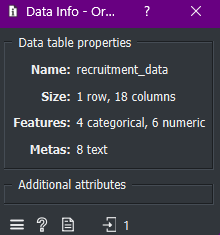
\includegraphics[width=13.5pc]{figures/DataInfo.png}}
% \caption{Basic Data Info about the data set from Orange.}
% \end{figure}



\section{Data cleaning}
\subsection{Missing Values}
While there are no officially recorded missing values in any of the columns, a more detailed examination of the {\it Phone Number} attribute reveals 400 hashed values, which can be considered as "disguised missing values."

\subsection{Duplicated Values}
There are no duplicated rows in the data set. 3,000 unique {\it Applicant ID}s, which span from 1001 to 4000, matching the data set's size.

\subsection{Changing Data Type}
{\it Application Date} and {\it Date of Birth} attributes that were in the object type are converted into date time type and in ISO format to maintain consistency and for analysis.

\section{Feature Engineering}
Feature engineering is the pre-processing step, which is used to transform raw data into features that can be used for creating a predictive model using machine learning or statistical modeling. \cite{c} However, three new attributes are created mostly for the purpose of visualization

\subsection{Age}
An attribute {\textit Age} is generated by taking the difference between {\it Application Date} and {\it Date of Birth}.

$$
Age = ApplicationDate - DateOfBirth
$$

\begin{table}[htbp]
  \centering
  \caption{Age Attribute}
    \begin{tabular}{c c c c}
    \hline
    Applicant ID & Application Date & Date of Birth & Age \\
    \hline
    1001 & 2023-06-03 & 1992-08-31 & 30 \\
    1002 & 2023-06-03 & 1965-04-29 & 58 \\
    1003 & 2023-08-04 & 1973-03-10 & 50 \\
    \hline
  \end{tabular}
\end{table}


\subsection{State}
The {\it State} attribute involves matching state abbreviations from the USA to their respective full state names. This process serves to confirm if all the states listed are indeed part of the United States, and it also enhances comprehension for the recruiter. The {\it StateName} attribute is created by utilizing a Python Dictionary containing a translation of US states into their corresponding two-letter codes.

\begin{table}[htbp]
  \centering
  \caption{StateName Attribute}
    \begin{tabular}{c c c c}
    \hline
    State & StateName \\
    \hline
    NV & Nevada \\
    TN & Tennessee \\
    TX & Texas \\
    \hline
  \end{tabular}
\end{table}

\section{More Data Cleaning}
\subsection{Location: State and Country}
The discrepancy arises when the applicants' states belong to the United States, but their countries do not match. This indicates an inconsistency in the location details provided by the applicants. To address this issue during analysis, the preferred location data to consider is either the State or StateName attribute from the applicant names.

\subsection{Years of Experience and Age}
In certain cases, there are applicants whose {\it Years of Experience} is significantly high compared to their {\it Age}. Additionally, there are instances where {\it Years of Experience} surpasses {\it Age}, which is logically implausible. This could be attributed to applicants potentially providing inaccurate information regarding their {\it Years of Experience}, or errors in data entry. It's important to note that, given the minimum federal working age in the USA (the applicants' country) is 14, we only analyze data where the age-experience difference is at least 14 years.



\section{EDA: Non-Graphical Method}
In non-graphical data analysis method, when dealing with categorical data, we perform cross-tabulation between two variables. In contrast, when working with numerical data, we rely on summary statistics and correlation analysis.

\subsection{Categorical}
Cross tabulation is done between two categorical attributes to determine the count between categories. Taking all results provides the tabulation of the frequency of each category. The method is done among categories such as {\it Education Level}, {\it Gender}, and {\it Status}.

\begin{table}[h]
  \centering
  \caption{Cross Tabulation of Education Level and Status}
  \resizebox{0.45\textwidth}{!}{%
    \begin{tabular}{c c c c c c c}
      \hline
      \textbf{Status} & \textbf{Applied} & \textbf{In Review} & \textbf{Interviewing} & \textbf{Offered} & \textbf{Rejected} & \textbf{All} \\
      \textbf{Education Level} \\
      \hline
      \textbf{Bachelor’s Degree} & 164 & 133 & 172 & 157 & 159 & 785 \\
      \textbf{High School} & 147 & 158 & 140 & 141 & 152 & 738 \\
      \textbf{Master’s Degree} & 149 & 149 & 137 & 164 & 137 & 736 \\
      \textbf{PhD} & 151 & 155 & 141 & 148 & 146 & 741 \\
      \hline
      \textbf{All} & 611 & 590 & 610 & 594 & 3000 \\
      \hline
    \end{tabular}%
  }
\end{table}

\begin{table}[h]
  \centering
  \caption{Cross Tabulation of Education Level and Gender}
    \begin{tabular}{c c c c c}
      \hline
      \textbf{Gender} & \textbf{Female} & \textbf{Male} & \textbf{Other} & \textbf{All} \\
      \textbf{Education Level} \\
      \hline
      \textbf{Bachelor’s Degree} & 265 & 260 & 260 & 785 \\
      \textbf{High School} & 234 & 267 & 237 & 738 \\
      \textbf{Master’s Degree} & 243 & 248 & 245 & 736  \\
      \textbf{PhD} & 225 & 255 & 261 & 741 \\
      \hline
      \textbf{All} & 967 & 1030 & 1003 & 3000 \\
      \hline
    \end{tabular}
\end{table}

\subsection{Quantitative}
To understand the distribution of numerical attributes like {\it Years of Experience}, {\it Desired Salary}, and {\it Age} we analyze their population characteristics. This includes examining central tendencies like the mean, median, and mode, as well as measures of spread such as standard deviation.

\begin{table}[htbp]
  \centering
  \caption{Statistical Summary of Uni-Variate Numeric Columns}
    \begin{tabular}{c c c c c}
      \hline
       & \textbf{Years of Experience} & \textbf{Desired Salary} & \textbf{Age} \\
      \hline
      \textbf{Count} & 3000.0 & 3000.0 & 3000.0 \\
      \textbf{Mean} & 10.0 & 65079.1 & 39.4  \\
      \textbf{Std. Deviation} & 6.0 & 20163.7 & 12.5 \\
      \textbf{Min} & 0.0 & 30047.2 & 17.0 \\
      \textbf{25\%} & 5.0 & 47307.8 & 29.0  \\
      \textbf{50\%} & 10.0 & 64934.9 & 40.0 \\
       \textbf{75\%} & 15.0 & 82585.6 & 50.01 \\
      \textbf{Max} & 20.0 & 99992.7 & 60 \\
      \hline
    \end{tabular}
\end{table}

We construct a matrix containing pairwise correlations to identify statistical associations. Based on TABLE VI, it is evident that there are no correlations among the attributes.

\begin{table}[htbp]
  \centering
  \caption{Correlation Matrix of Numeric Columns}
    \begin{tabular}{c c c c c}
      \hline
       & \textbf{Years of Experience} & \textbf{Desired Salary} & \textbf{Age} \\
      \hline
      \textbf{Years of Experience} & 1.0 & 0.028 & 0.22 \\
      \textbf{Desired Salary} & 0.028 & 1.0 & -0.0091  \\
      \textbf{Age} & 0.22 & -0.0091 & 1.0 \\
      \hline
    \end{tabular}
\end{table}

\begin{figure} [htbp]
\centerline{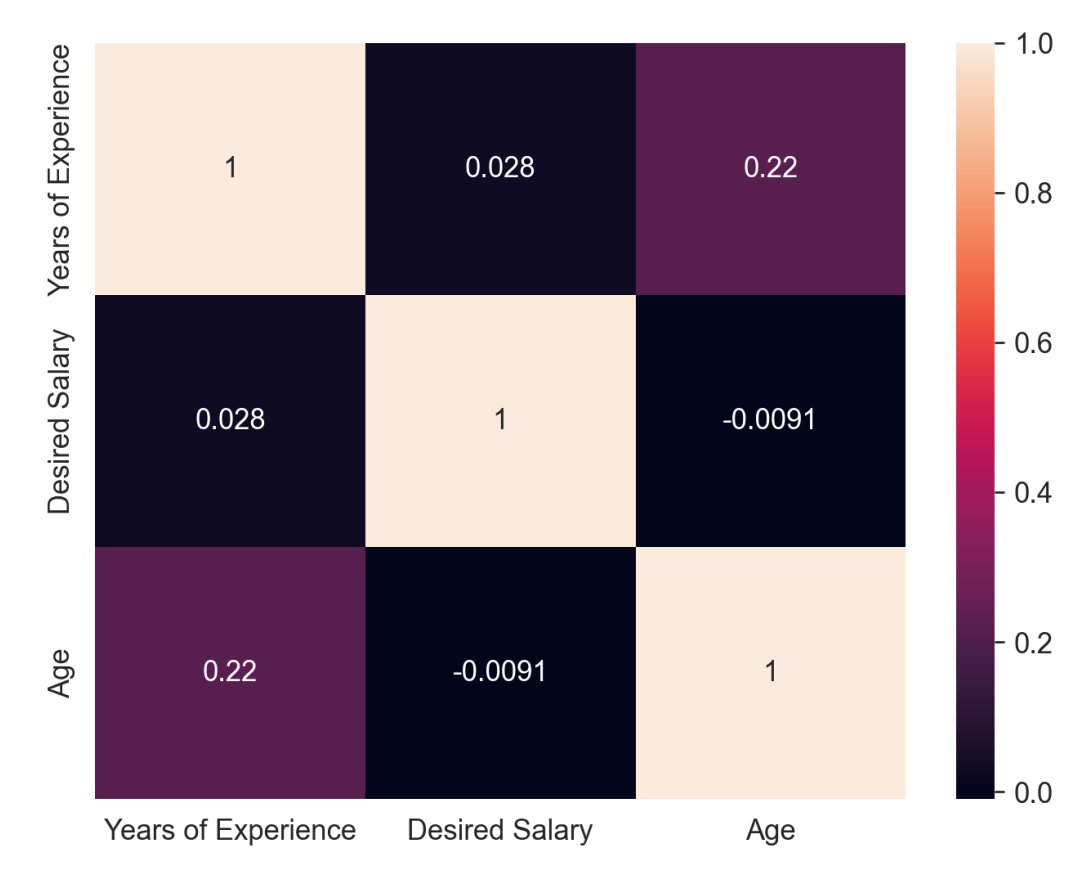
\includegraphics[width=16.5pc]{figures/HeatMap.png}}
\caption{Heatmap of Correlation Matrix shown in TABLE VI.}
\end{figure}



\section{EDA: Graphical Method}
To gain insights from the data and extract valuable information, we can employ a range of visualizations, including distribution plots, categorical plots, matrix plots, and relational plots. These visual representations help us better understand and analyze the data.

\subsection{Distribution Plot}
In distribution plots, we create histograms and kernel density estimator (KDE) plots to determine the data's distribution characteristics, such as whether it follows a uniform distribution or exhibits left or right skewness.

\begin{figure}
\centerline{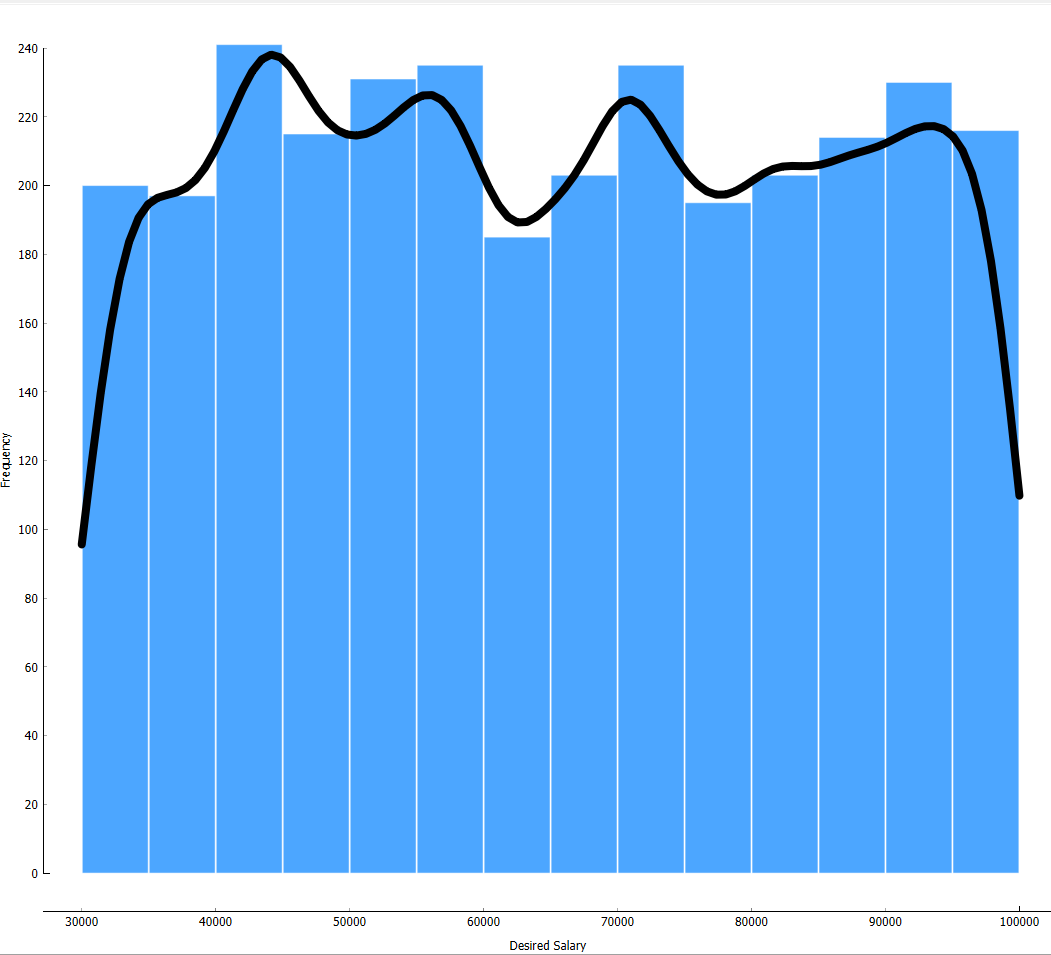
\includegraphics[width=16.5pc]{figures/desiredSalaryN.png}}
\caption{Distribution of Desired Salary with KDE (Binwidth: 5000).}
\end{figure}


{\it Fig 2.} shows that the applicant's desired salary is uniform and ranges from 300047.2 to 99992.7.



\begin{figure}[h]
\centerline{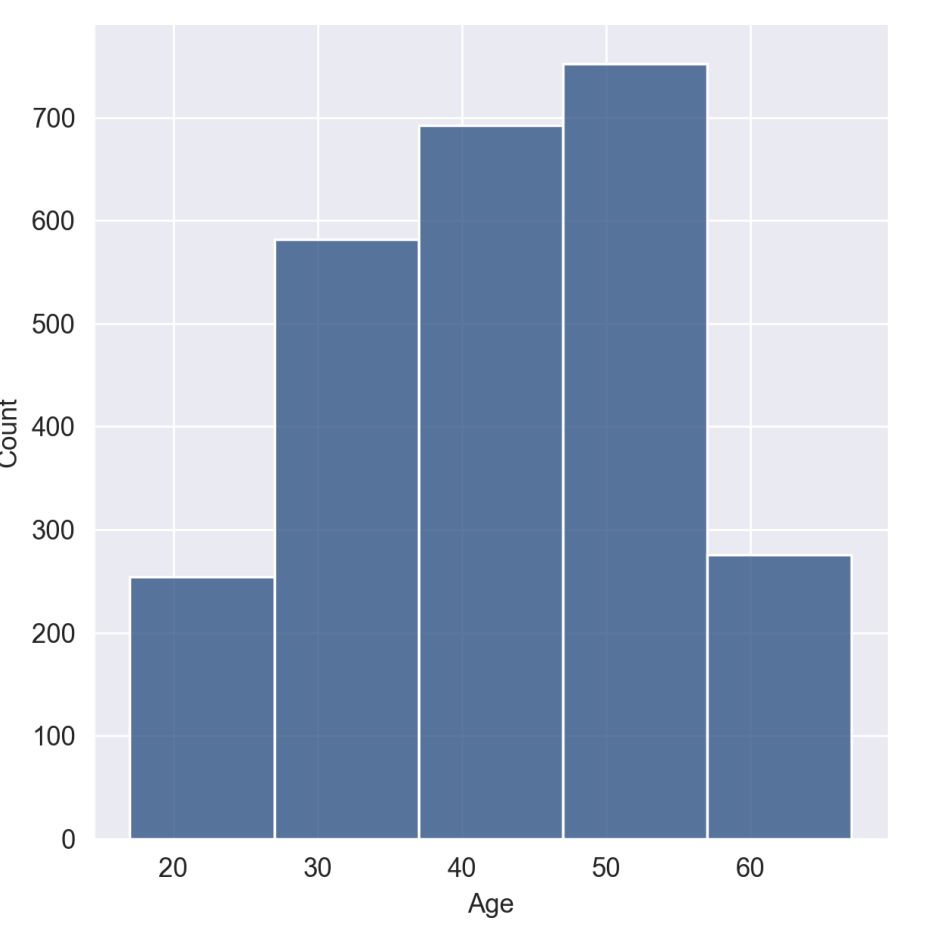
\includegraphics[width=16.5pc]{figures/age-distribution.png}}
\caption{Distribution of Age (Binwidth: 5).}
\end{figure}

{\it Fig 3.} illustrates that the age of applicants spans from 20 to 60, with the majority falling within the 30-50 age range. This analysis suggests that individuals in their 20s are beginning their careers in the job market, while those in their 60s are typically retiring from their professions.

\subsection{Categorical Plot}
Categorical plots offer various ways to represent data, including counting category occurrences, depicting categorical attributes based on values with aggregation, and combining categorical and numerical attributes through plots like box plots and line charts.

\begin{figure}[htbp]
\centerline{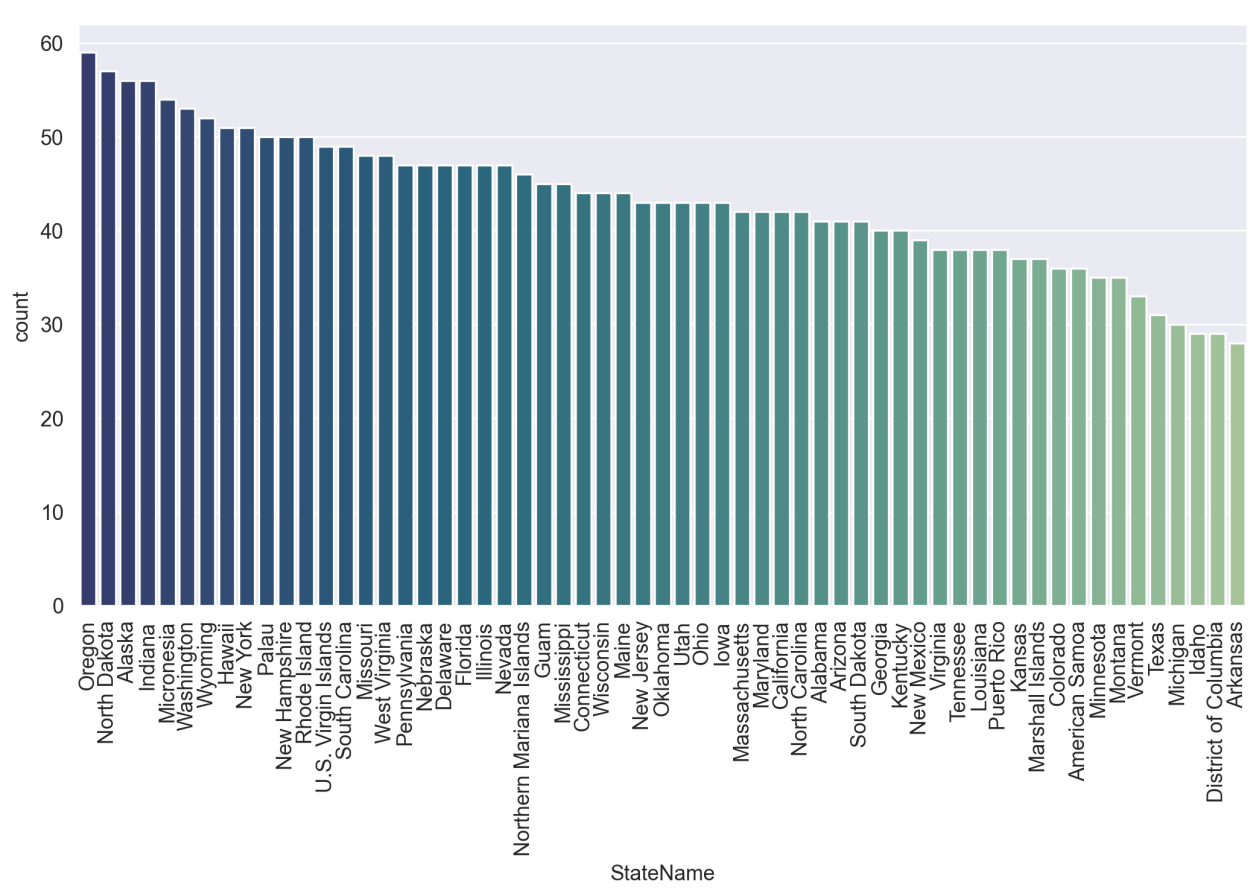
\includegraphics[width=20pc]{figures/state-distributionN.png}}
\caption{Distribution of Applicants based on State.}
\end{figure}

{\it Fig 4.} indicates that the largest number of applicants originate from Oregon and North Dakota states, while the smallest number come from Arkansas.


\begin{figure}[htbp]
\centerline{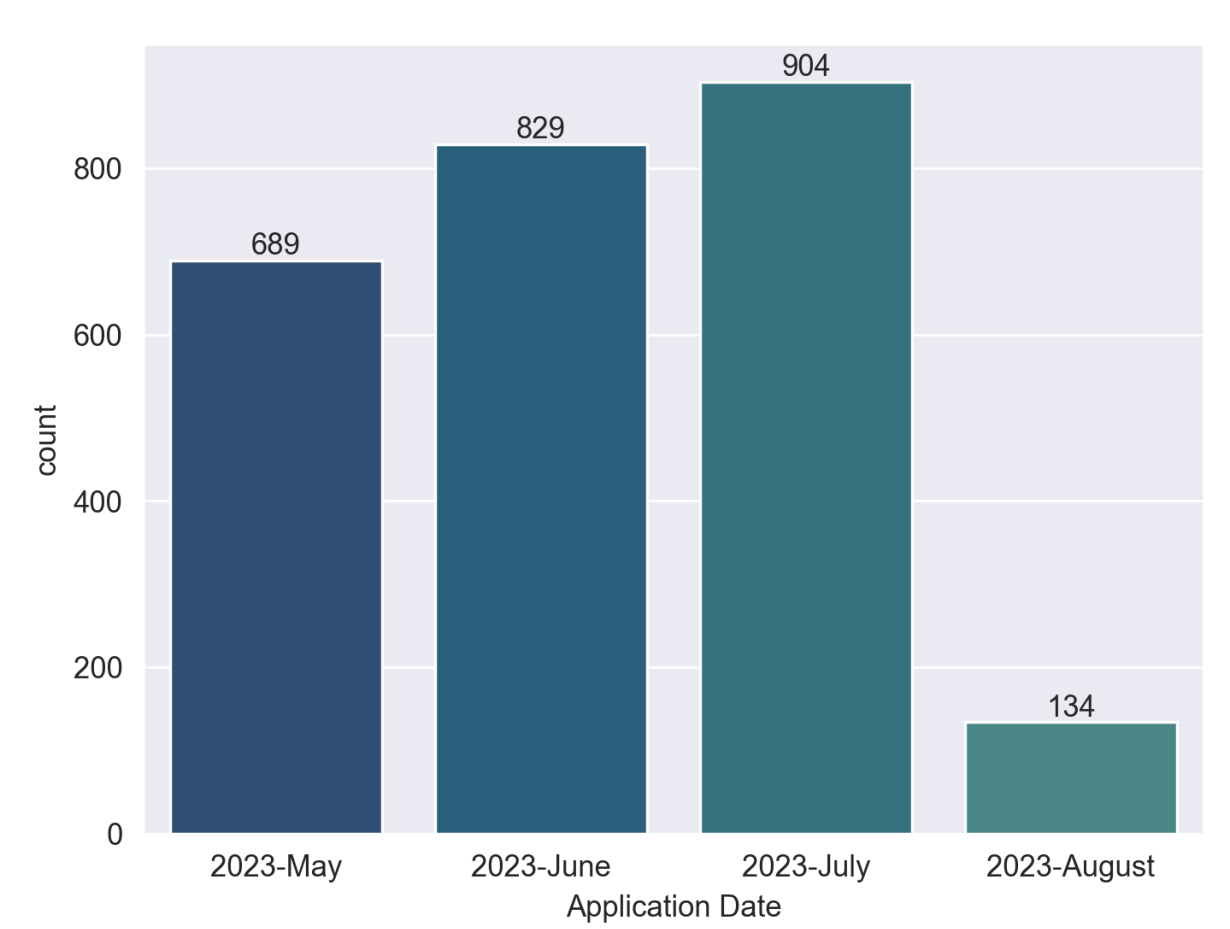
\includegraphics[width=16.5pc]{figures/applicantdate-N.png}}
\caption{Frequency of Applicant’s based on Months.}
\end{figure}

{\it Fig 5.} displays the applicant count from May 2023 to August 2023. It is evident that the highest number of applicants occurred in July, followed by a significant decrease in August.
\clearpage


\begin{figure}
\centerline{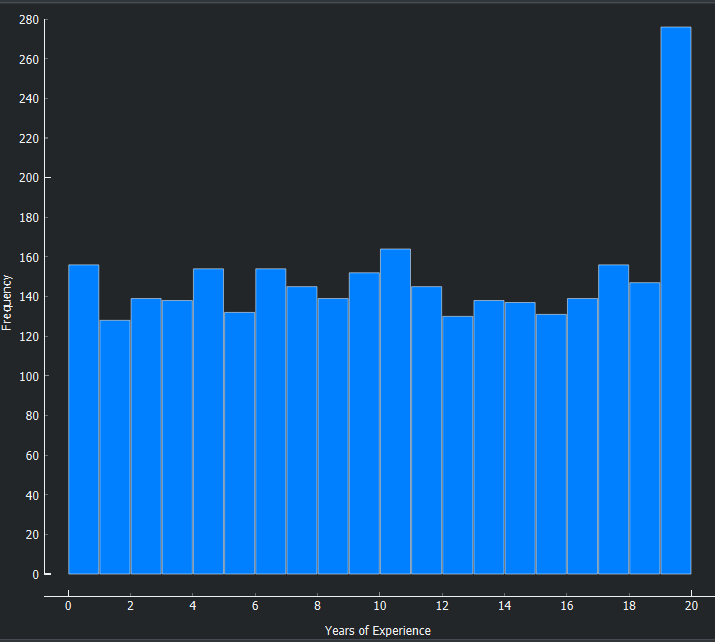
\includegraphics[width=16.5pc]{figures/Distribution-YearsOfExperience.png}}
\caption{Distribution of Years of Experience.}
\end{figure}
{\it Fig 6.} shows the frequency distribution of applicants according to their years of experience. The graph shows that most of the applicants have 20 years of experience.



\begin{figure}[htbp]
\centerline{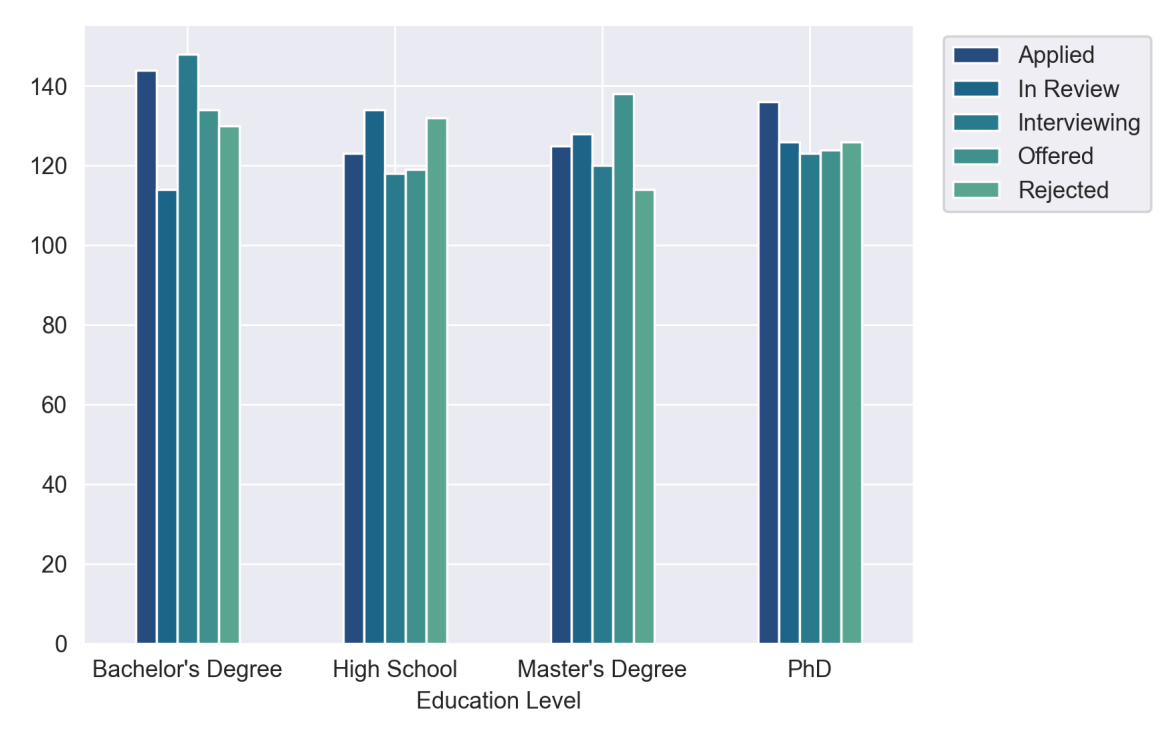
\includegraphics[width=17.5pc]{figures/educationlevelandstatusN.png}}
\caption{Box plot for different education levels based on the desired salary.}
\end{figure}

{\it Fig 7.} shows visualization of the cross-tabulation of {\it Education Level} and {\it Status} that was performed in TABLE III. We can see that the highest number of applicants interviewed are from Bachelor’s Degrees, and those rejected are from High School and Bachelor’s Degrees.


\begin{figure}[htbp]
\centerline{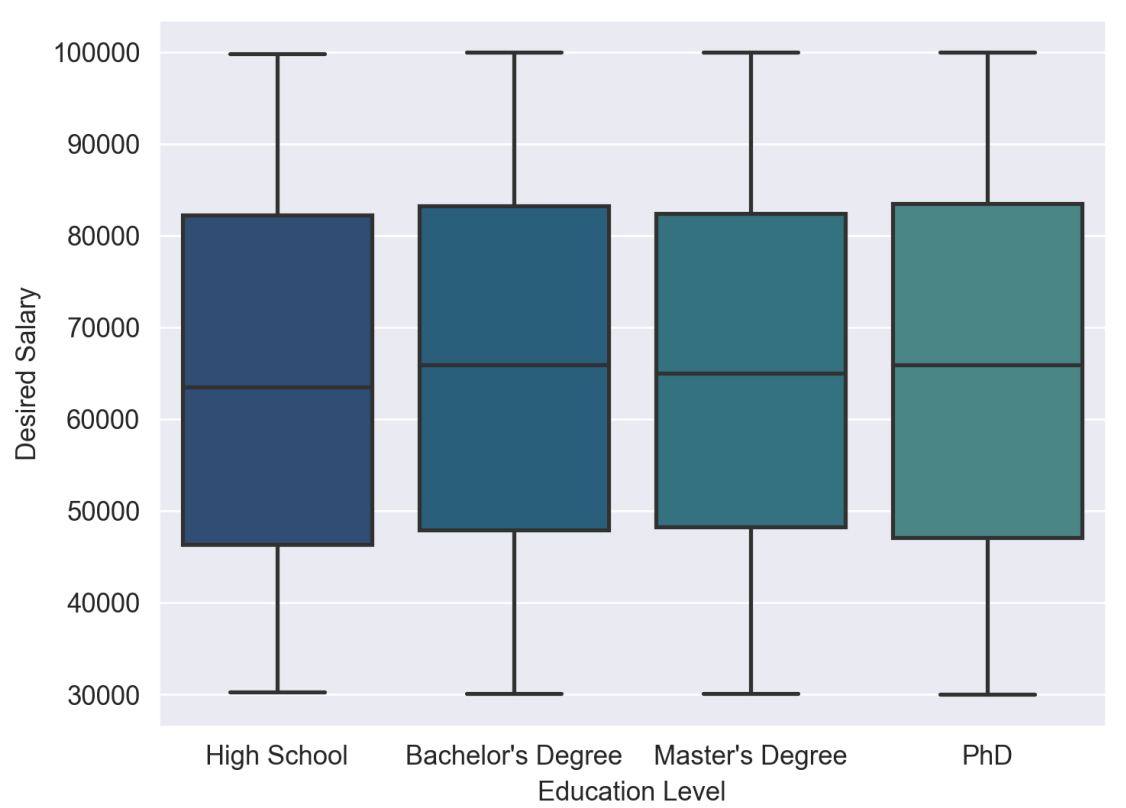
\includegraphics[width=17.5pc]{figures/box-whisker.png}}
\caption{Box plot for different education levels based on the desired salary.}
\end{figure}

{\it Fig 8.} illustrates that the median desired salary for all education levels is similar, and no outliers are detected in the desired salary data.


\begin{figure}[h]
\centerline{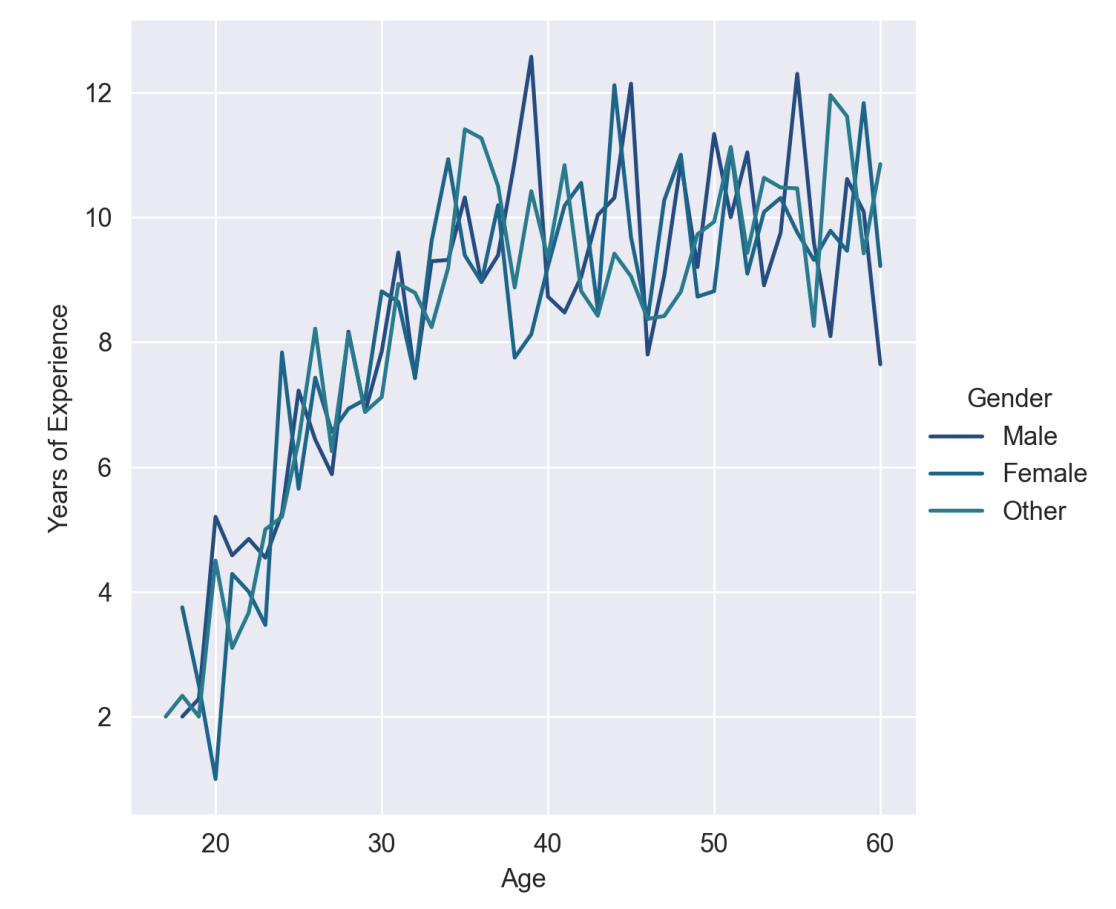
\includegraphics[width=16.5pc]{figures/LineChartN.png}}
\caption{Line chart showing years of experiences of different age group as their age increases.}
\end{figure}

{\it Fig 9.} demonstrates a positive correlation between an applicant's age and their years of experience, which aligns with the expected trend.













\section{Conclusion}
Our analysis involved an extensive exploration of the recruitment dataset, wherein we not only conducted exploratory data analysis but also implemented a diverse set of preprocessing techniques. Through this comprehensive approach, we've uncovered notable patterns and trends that could prove to be invaluable insights for the organization's decision-making processes. These findings have the potential to inform and guide future strategies related to recruitment and talent acquisition, ultimately contributing to the organization's overall success.


\section*{Acknowledgment}
I would like to express my sincere gratitude to Asst. Prof. Rajani Chulyadyo for providing me with the data set used in this EDA report. Her teaching and support were instrumental in the successful completion of this analysis. I also want to acknowledge my classmates for guiding me throughout and providing valuable resources during this research.



% \begin{thebibliography}{34}\vspace*{-12pt}

% \bibitem{}G. O. Young, ``Synthetic structure of industrial plastics,'' in {\em Plastics},\break 2nd ed., vol. 3, J. Peters, Ed. New York, NY, USA: McGraw-Hill, 1964,\break pp. 15--64.

% \bibitem{}W.-K. Chen, {\it Linear Networks and Systems}. Belmont, CA, USA: Wadsworth, 1993, pp. 123--135.

% \end{thebibliography}

% \subsection*{Basic format for books:}\vspace*{-12pt}
% \def\refname{}
% \begin{thebibliography}{34}
% \item[] J. K. Author, ``Title of chapter in the book,'' in {\em Title of His Published Book}, xth ed. City of Publisher, (only U.S. State), Country: Abbrev. of Publisher, year, ch. x, sec. x, pp. xxx--xxx.
% \end{thebibliography}




% \subsection*{Examples:}


% \bibitem{}G. O. Young, ``Synthetic structure of industrial plastics,'' in {\em Plastics},\break 2nd ed., vol. 3, J. Peters, Ed. New York, NY, USA: McGraw-Hill, 1964,\break pp. 15--64.


\section*{References}


\def\refname{}
\begin{thebibliography}{34}\vspace*{-12pt}
\bibitem{a} KnowledgeHut. (2023). Exploratory Data Analysis (EDA): Types, Tools, Process. [Online]. Available: \url{https://www.knowledgehut.com/blog/data-science/eda-data-science}. [Accessed 10 Sep. 2023].

\bibitem{b} A Horsch. (2023). Hypothesis testing for data scientists. [Online]. Available: \url{https://towardsdatascience.com/hypothesis-testing-for-data-scientists-everything-you-need-to-know-8c3}\break\url{6ddde4cd2}. [Accessed 10 Sep. 2023].

\bibitem{c} JavaTpoint. (2023). Feature Engineering for Machine Learning. [Online]. Available: \url{https://www.javatpoint.com/feature-engineering-for-machine-learning}. [Accessed 10 Sep. 2023].
\end{thebibliography}


% \def\refname{}




% \subsection*{Basic format for reports:}\vspace*{-12pt}
% \begin{thebibliography}{34}
% \item[]
% J. K. Author, ``Title of report,'' Abbrev. Name of Co., City of Co., Abbrev. State, Country, Rep. xxx, year.
% \end{thebibliography}

% \subsection*{Examples:}\vspace*{-12pt}
% \begin{thebibliography}{34}
% \setcounter{enumiv}{5}

% \bibitem{} E. E. Reber, R. L. Michell, and C. J. Carter, ``Oxygen absorption in the earth’s atmosphere,'' Aerospace Corp., Los Angeles, CA, USA, Tech. Rep. TR-0200 (4230-46)-3, Nov. 1988.

% \bibitem{} J. H. Davis and J. R. Cogdell, ``Calibration program for the 16-foot antenna,'' Elect. Eng. Res. Lab., Univ. Texas, Austin, TX, USA, Tech. Memo. NGL-006-69-3, Nov. 15, 1987.
% \end{thebibliography}


% \subsection*{Basic format for books (when available online):}\vspace*{-12pt}
% \begin{thebibliography}{34}
% \item[]
% J. K. Author, ``Title of chapter in the book,'' in {\em Title of Published Book}, xth ed. City of Publisher, State, Country: Abbrev. of Publisher, year, ch. x, sec. x, pp. xxx--xxx. [Online]. Available: http://www.web.com 
% \end{thebibliography}


% \subsection*{Examples:}\vspace*{-12pt}

% \begin{thebibliography}{34}
% \setcounter{enumiv}{9}

% \bibitem{}G. O. Young, ``Synthetic structure of industrial plastics,'' in Plastics, vol. 3, Polymers of Hexadromicon, J. Peters, Ed., 2nd ed. New York, NY, USA: McGraw-Hill, 1964, pp. 15--64. [Online]. Available: http://www.bookref.com. 

% \bibitem{} {\em The Founders Constitution}, Philip B. Kurland and Ralph Lerner, eds., Chicago, IL, USA: Univ. Chicago Press, 1987. [Online]. Available: http://press-pubs.uchicago.edu/founders/

% \bibitem{} The Terahertz Wave eBook. ZOmega Terahertz Corp., 2014. [Online]. Available: http://dl.z-thz.com/eBook/zomega\_ebook\_pdf\_1206\_sr.pdf. Accessed on: May 19, 2014. 

% \bibitem{} Philip B. Kurland and Ralph Lerner, eds., {\em The Founders Constitution}. Chicago, IL, USA: Univ. of Chicago Press, 1987, Accessed on: Feb. 28, 2010, [Online] Available: http://press-pubs.uchicago.edu/founders/ 
% \end{thebibliography}

% \subsection*{Basic format for journals (when available online):}\vspace*{-12pt}
% \begin{thebibliography}{34}
% \item[] J. K. Author, ``Name of paper,'' {\em Abbrev. Title of Periodical}, vol. x, no. x, pp. xxx--xxx, Abbrev. Month, year. Accessed on: Month, Day, year, DOI: 10.1109.XXX.123456, [Online].
% \end{thebibliography}

% \subsection*{Examples:}\vspace*{-12pt}

% \begin{thebibliography}{34}
% \setcounter{enumiv}{13}

% \bibitem{}J. S. Turner, ``New directions in communications,'' {\em IEEE J. Sel. Areas Commun.}, vol. 13, no. 1, pp. 11--23, Jan. 1995. 

% \bibitem{} W. P. Risk, G. S. Kino, and H. J. Shaw, ``Fiber-optic frequency shifter using a surface acoustic wave incident at an oblique angle,'' {\em Opt. Lett.}, vol. 11, no. 2, pp. 115--117, Feb. 1986.

% \bibitem{} P. Kopyt {\em et al.}, ``Electric properties of graphene-based conductive layers from DC up to terahertz range,'' {\em IEEE THz Sci. Technol.}, to be published. DOI: \href{https://dx.doi.org/10.1109.XXX.123456}{10.1109/TTHZ.2016.2544142}.
% \end{thebibliography}

% \subsection*{Example when using et al.:}\vspace*{-18pt}

% \begin{thebibliography}{34}
% \setcounter{enumiv}{33}

% \bibitem{}S. Azodolmolky {\em et al.}, ``Experimental demonstration of an impairment aware network planning and operation tool for transparent/translucent optical networks,'' {\em J. Lightw. Technol.}, vol. 29, no. 4, pp. 439--448, Sep. 2011.
% \end{thebibliography}







% \section{Guidelines For Graphics Preparation and Submission}

% \subsection{Types of Graphics}

% The following list outlines the different types of graphics published in IEEE journals. They are categorized based on their construction, and use of color / shades\vadjust{\pagebreak} of gray:

% \begin{enumerate}
% \item[{\it 1)}]{\it Color/Grayscale Figures}

% Figures that are meant to appear in color, or shades of black/gray. Such figures may include photographs, illustrations, multicolor graphs, and flowcharts.

% \item[{\it 2)}]{\it Line Art Figures}

% Figures that are composed of only black lines and shapes. These figures should have no shades or half-tones of gray, only black and white.

% \item[{\it 3)}]{\it Author Photos}

% Head and shoulders shots of authors that appear at the end of our papers.

% \item[{\it 4)}]{\it Tables}

% Data charts which are typically black and white, but sometimes include color.
% \end{enumerate}




\end{document}
